\chapter{Química do estado sólido: bandas, defeitos e semicondutores}\label{ch:b3:solid-state}

Um painel solar em um telhado e o diodo emissor de luz de uma lâmpada são feitos do
mesmo tipo de cristal, silício ou um composto de gálio com nitrogênio, arsênio
ou fósforo, no qual se colocaram de propósito alguns átomos de impureza por
milhão. Seu funcionamento é fixado por duas coisas que uma molécula não tem: bandas de
níveis de energia, com uma \omterm{def:b3:solid-state:band}{banda proibida} cuja largura fixa qual luz um cristal absorve ou
emite, e defeitos, que transportam as cargas. Este capítulo constrói as bandas
a partir dos orbitais moleculares, conta os portadores de um \omterm{def:b3:solid-state:classes}{semicondutor} e trata
os átomos ausentes ou fora de lugar como espécies químicas com seus próprios equilíbrios,
até o \omterm{def:b3:solid-state:ionic-conductor}{eletrólito sólido} do sensor de oxigênio no escapamento de um carro.

\begin{recall}
O volume do 1.º ano definiu os cristais, a ligação metálica, os cristais iônicos e
covalentes, os sítios intersticiais e as ligas, e a equação de Nernst; o volume do 2.º
ano, o método de Hückel e a integral de ressonância $\beta$.
O \cref{ch:b3:x-ray-diffraction} deu a \omterm{def:b3:x-ray-diffraction:reciprocal}{rede recíproca} e o
\cref{ch:b3:partition-functions}, a \omterm{def:b3:partition-functions:boltzmann}{distribuição de Boltzmann} e a
\omterm{def:b3:partition-functions:statistical-entropy}{entropia estatística} $S = k\ln W$.
\end{recall}

\begin{omfigure}
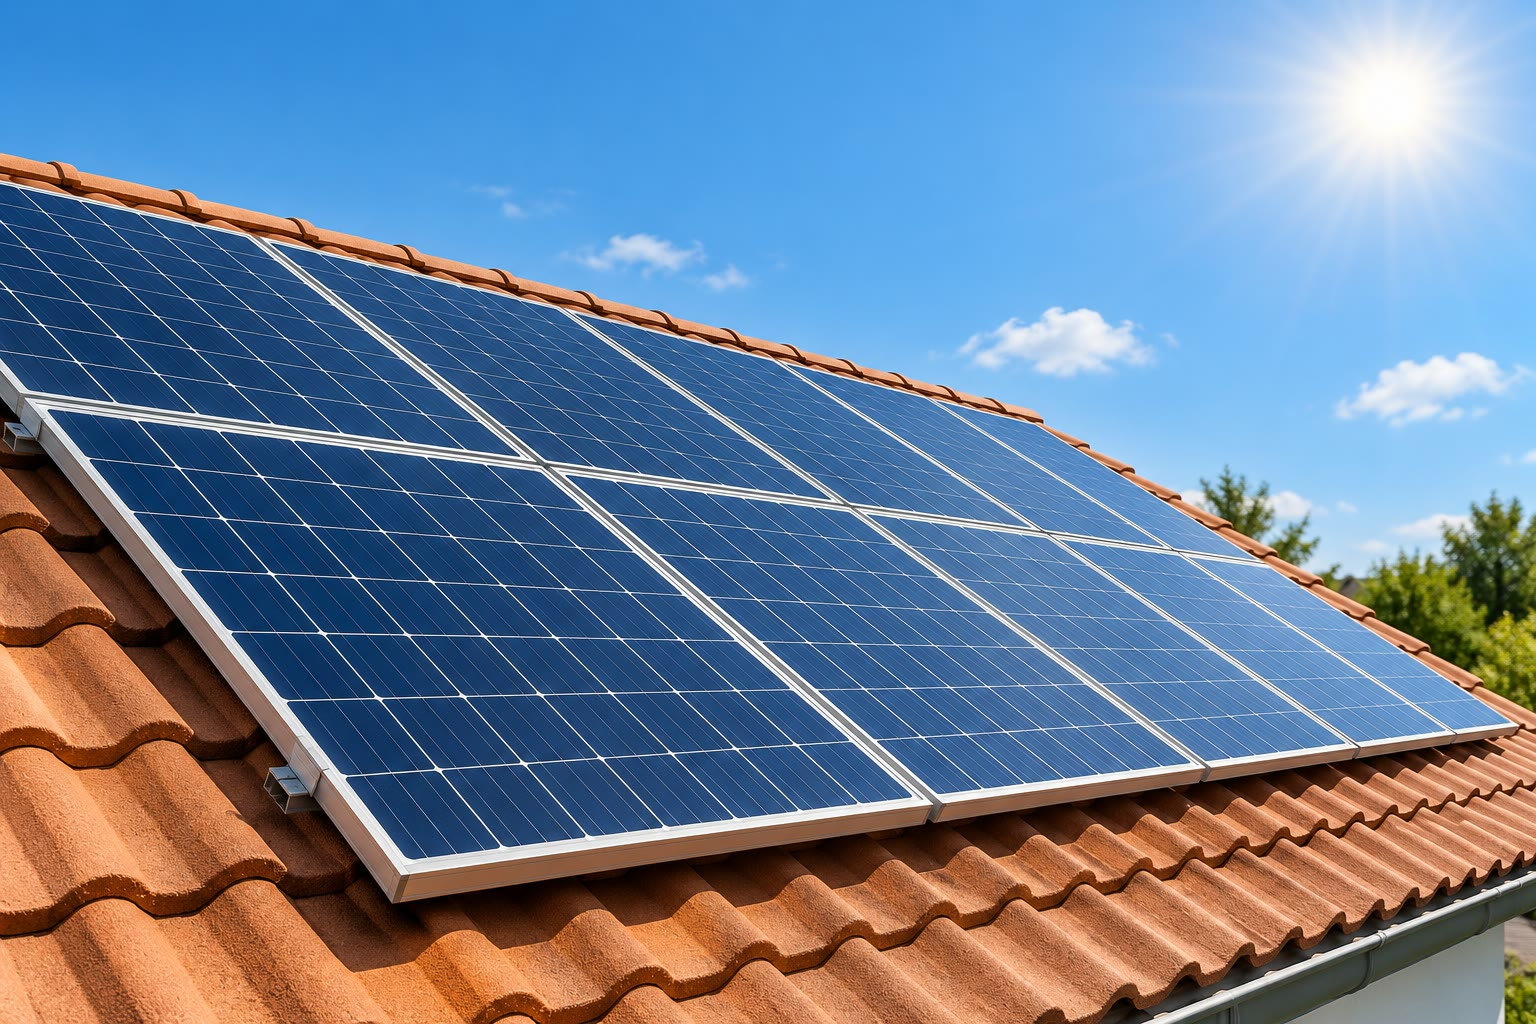
\includegraphics[width=0.6\linewidth]{images/book4/ai/b3-22-solar-panels.jpg}

{\small Painéis solares em um telhado de telhas: cada célula é uma fina fatia de silício
na qual a luz eleva elétrons através de uma \omterm{def:b3:solid-state:band}{banda proibida} de cerca de um elétron-volt.}
\end{omfigure}

\section{Dos orbitais às bandas}

Tome uma cadeia de $N$ átomos idênticos, cada um com um orbital s, na aproximação de
Hückel: integral de Coulomb $\alpha$ em cada átomo, integral de ressonância $\beta < 0$
entre vizinhos, zero nos demais casos.

\begin{theorem}[Níveis de uma cadeia de Hückel]\label{thm:b3:solid-state:chain}
Os $N$ orbitais moleculares de uma cadeia linear de $N$ átomos têm energias
\[
  E_k = \alpha + 2\beta\cos\frac{k\pi}{N + 1}, \qquad k = 1, \dots, N,
\]
com coeficientes $c_j^{(k)} \propto \sin\bigl(jk\pi/(N + 1)\bigr)$ no átomo $j$. Quando $N \to \infty$, os níveis preenchem
densamente o intervalo de $\alpha + 2\beta$ a $\alpha - 2\beta$: uma banda de largura $4|\beta|$.
\end{theorem}

\begin{proof}
As equações seculares são $\beta c_{j-1} + (\alpha - E)c_j + \beta c_{j+1} = 0$ para $j = 1, \dots, N$, com $c_0 = c_{N+1} = 0$
(não há átomo ali). Tente $c_j = \sin(j\theta)$: como $\sin((j - 1)\theta) + \sin((j + 1)\theta) = 2\cos\theta\sin(j\theta)$, cada
equação se torna $(\alpha - E + 2\beta\cos\theta)\sin(j\theta) = 0$, logo $E = \alpha + 2\beta\cos\theta$. A condição $c_0 = 0$ vale
para todo $\theta$, e $c_{N+1} = \sin((N + 1)\theta) = 0$ exige $\theta = k\pi/(N + 1)$; $k = 1, \dots, N$ dá $N$ níveis
distintos (os outros os repetem ou se anulam). O mais baixo e o mais alto são
$\alpha \pm 2\beta\cos(\pi/(N + 1))$, que tendem a $\alpha \pm 2\beta$; o espaçamento entre vizinhos é no máximo
$2|\beta|\pi/(N + 1)$, que tende a zero.
\end{proof}

Para $N = 2$, o teorema dá $\alpha \pm \beta$, os orbitais do sistema $\pi$ do eteno; para
$N = 6$, o hexatrieno de cadeia aberta. Em três dimensões, o mesmo ocorre com
todo tipo de orbital atômico: os orbitais s dão uma banda s, os orbitais p uma banda p,
e cada banda comporta $2N$ elétrons para $N$ átomos.

\begin{definition}[Bandas]\label{def:b3:solid-state:band}
Uma \emph{banda de energia}\index{banda de energia} de um cristal é um intervalo contínuo de
energias monoeletrônicas permitidas, formado a partir dos orbitais de todos os seus átomos. Uma
\emph{banda proibida}\index{banda proibida} $E_g$ é um intervalo de energias sem nenhum nível entre duas
bandas. Em um \omterm{def:b3:solid-state:classes}{semicondutor} ou em um \omterm{def:b3:solid-state:classes}{isolante} à temperatura zero, a banda preenchida
mais alta é a \emph{banda de valência}\index{banda de valencia@banda de valência} e a banda vazia mais
baixa, a \emph{banda de condução}\index{banda de conducao@banda de condução}.
\end{definition}

\begin{definition}[Densidade de estados e nível de Fermi]\label{def:b3:solid-state:fermi}
A \emph{densidade de estados}\index{densidade de estados} $g(E)$ é o número de
níveis por unidade de energia (e por átomo ou por unidade de volume) perto da energia $E$.
O \emph{nível de Fermi}\index{nivel de Fermi@nível de Fermi} $E_F$ é a energia na qual um nível tem
probabilidade $1/2$ de estar ocupado; à temperatura zero, todos os níveis abaixo dele estão
preenchidos e todos os acima, vazios.
\end{definition}

\begin{omfigure}
\begin{tikzpicture}
\begin{axis}[width=0.78\linewidth, height=6.2cm, xmin=0.3, xmax=7.6, ymin=-2.3, ymax=2.3,
  axis lines=left, xtick={1,2,3,4,5,6.6}, xticklabels={2,4,8,16,64,$\infty$: $g(E)$},
  xlabel={número de átomos $N$}, ylabel={$(E - \alpha)/|\beta|$},
  ytick={-2,-1,0,1,2}, tick label style={font=\small}, label style={font=\small}]
\addplot[only marks, mark=-, mark size=7pt, omDef, thick] table[x=col, y=e] {figdata/out/bachelor-3-band-chain.dat};
\addplot[omThm, thick] table[x expr=6.0+0.55*\thisrow{g}, y=e] {figdata/out/bachelor-3-band-chain-b.dat};
\draw[black!40, dashed] (axis cs:0.3,-2) -- (axis cs:7.6,-2);
\draw[black!40, dashed] (axis cs:0.3,2) -- (axis cs:7.6,2);
\draw[<->, black!60] (axis cs:5.6,-2) -- (axis cs:5.6,2) node[midway, left, font=\scriptsize] {$4|\beta|$};
\end{axis}
\end{tikzpicture}

{\small Níveis de Hückel de cadeias de 2 a 64 átomos (um traço curto por nível;
com $\beta < 0$, os níveis ligantes ficam embaixo). Os níveis se adensam em uma banda
entre $\alpha + 2\beta$ e $\alpha - 2\beta$; à direita, a \omterm{def:b3:solid-state:fermi}{densidade de estados} da cadeia
infinita, máxima nas bordas da banda.}
\end{omfigure}

\begin{proposition}[Preenchimento das bandas]\label{prop:b3:solid-state:filling}
Um cristal cuja banda ocupada mais alta está parcialmente preenchida conduz eletricidade
como um metal; um cristal cujas bandas estão cheias ou vazias, com uma \omterm{def:b3:solid-state:band}{banda proibida}
entre elas, não conduz à temperatura zero.
\end{proposition}

\begin{proof}[Argumento]
Em um campo elétrico, os elétrons ganham um pouco de energia e de momento: precisam
passar para níveis vazios logo acima dos que ocupam. Em uma banda parcialmente
preenchida, esses níveis ficam imediatamente acima do \omterm{def:b3:solid-state:fermi}{nível de Fermi}, sem custo de energia. Em
uma banda cheia, todo nível está ocupado e o próximo nível vazio fica do outro lado da \omterm{def:b3:solid-state:band}{banda proibida};
além disso, uma banda cheia não transporta corrente líquida, pois para cada elétron que se move
em um sentido outro se move no sentido oposto.
\end{proof}

O sódio, com um elétron 3s por átomo, preenche metade de sua banda s: um metal.
O magnésio, com dois, preencheria exatamente sua banda s, mas as bandas s e p
se sobrepõem, de modo que ele também é um metal. O diamante e o silício têm quatro elétrons de valência
por átomo em orbitais que se desdobram em uma banda ligante cheia e uma banda
antiligante vazia, separadas por uma \omterm{def:b3:solid-state:band}{banda proibida}.

\begin{definition}[Semicondutores e isolantes]\label{def:b3:solid-state:classes}
Um \emph{semicondutor}\index{semicondutor} é um sólido com uma \omterm{def:b3:solid-state:band}{banda proibida} pequena
o bastante (até cerca de \qty{3}{eV}) para que um número mensurável de elétrons a atravesse
à temperatura ambiente ou após dopagem; um \emph{isolante}\index{isolante}
tem uma \omterm{def:b3:solid-state:band}{banda proibida} tão larga que não conduz.
\end{definition}

\begin{omfigure}
\begin{tikzpicture}[font=\small]
  \foreach \x/\name in {0/metal, 3.6/semicondutor, 7.2/isolante} {
    \node[font=\small\bfseries] at (\x+0.8,4.3) {\name};
  }
  % metal: one partly filled band
  \fill[omDef!55] (0,0.4) rectangle (1.6,2.0);
  \draw (0,0.4) rectangle (1.6,3.4);
  \draw[omThm, thick] (-0.25,2.0) -- (1.85,2.0) node[right, font=\scriptsize] {$E_F$};
  % semiconductor: small gap
  \fill[omDef!55] (3.6,0.4) rectangle (5.2,1.7);
  \draw (3.6,0.4) rectangle (5.2,1.7);
  \draw (3.6,2.5) rectangle (5.2,3.8);
  \draw[omThm, thick] (3.35,2.1) -- (5.45,2.1) node[right, font=\scriptsize] {$E_F$};
  \draw[<->] (4.4,1.7) -- (4.4,2.5) node[pos=0.8, right, font=\scriptsize] {$E_g$};
  % insulator: large gap
  \fill[omDef!55] (7.2,0.4) rectangle (8.8,1.2);
  \draw (7.2,0.4) rectangle (8.8,1.2);
  \draw (7.2,3.2) rectangle (8.8,4.0);
  \draw[omThm, thick] (6.95,2.2) -- (9.05,2.2) node[right, font=\scriptsize] {$E_F$};
  \draw[<->] (8.0,1.2) -- (8.0,3.2) node[pos=0.75, right, font=\scriptsize] {$E_g$};
  \node[font=\scriptsize, anchor=east] at (3.5,1.05) {valência};
  \node[font=\scriptsize, anchor=east] at (3.5,3.15) {condução};
  \draw[->] (-0.6,0.2) -- (-0.6,3.9) node[above, font=\scriptsize] {$E$};
\end{tikzpicture}

{\small Preenchimento das bandas à temperatura zero (níveis preenchidos sombreados). Um metal tem uma
banda parcialmente preenchida e seu \omterm{def:b3:solid-state:fermi}{nível de Fermi} dentro dela; um \omterm{def:b3:solid-state:classes}{semicondutor} e um
\omterm{def:b3:solid-state:classes}{isolante} têm uma \omterm{def:b3:solid-state:band}{banda de valência} cheia e uma \omterm{def:b3:solid-state:band}{banda de condução} vazia, com o \omterm{def:b3:solid-state:fermi}{nível de
Fermi} na \omterm{def:b3:solid-state:band}{banda proibida}, estreita no primeiro e larga no segundo.}
\end{omfigure}

\section{Semicondutores}

\begin{definition}[Portadores]\label{def:b3:solid-state:carriers}
Um \emph{semicondutor intrínseco}\index{semicondutor intrinseco@semicondutor intrínseco} é um
\omterm{def:b3:solid-state:classes}{semicondutor} puro, cujos portadores vêm todos de elétrons excitados através da \omterm{def:b3:solid-state:band}{banda proibida}. Um
\emph{portador de carga}\index{portador de carga} é uma partícula móvel que transporta
corrente: um elétron na \omterm{def:b3:solid-state:band}{banda de condução}, ou um \emph{buraco}\index{buraco}, um
nível vazio na \omterm{def:b3:solid-state:band}{banda de valência}, que se move como uma carga positiva.
\end{definition}

\begin{theorem}[Concentração de portadores intrínsecos]\label{thm:b3:solid-state:intrinsic}
Com $N_c$ e $N_v$ as \omterm{def:b3:solid-state:fermi}{densidades de estados} efetivas das \omterm{def:b3:solid-state:band}{bandas de condução} e de
valência (admitidas), as concentrações de elétrons e de \omterm{def:b3:solid-state:carriers}{buracos} de um \omterm{def:b3:solid-state:classes}{semicondutor}
cujo \omterm{def:b3:solid-state:fermi}{nível de Fermi} está a mais de alguns $kT$ de cada borda de banda são
\[
  n = N_c\,\eu^{-(E_c - E_F)/kT}, \qquad p = N_v\,\eu^{-(E_F - E_v)/kT},
\]
e, em um \omterm{def:b3:solid-state:carriers}{semicondutor intrínseco},
\[
  n = p = n_i = \sqrt{N_cN_v}\,\eu^{-E_g/2kT}.
\]
\end{theorem}

\begin{proof}
A ocupação de um nível de energia $E$ é $f(E) = 1/(1 + \eu^{(E - E_F)/kT})$. Quando
$E - E_F \gg kT$, $f \approx \eu^{-(E - E_F)/kT}$, uma cauda de Boltzmann. Somando-a sobre os níveis da \omterm{def:b3:solid-state:band}{banda de
condução}, $n = \int g_c(E)\eu^{-(E - E_F)/kT}\,\dd E = \eu^{-(E_c - E_F)/kT}\int g_c(E)\eu^{-(E - E_c)/kT}\,\dd E$, e a última integral é por
definição $N_c$. Os \omterm{def:b3:solid-state:carriers}{buracos} são níveis vazios, com probabilidade $1 - f \approx \eu^{-(E_F - E)/kT}$ na
\omterm{def:b3:solid-state:band}{banda de valência}; as mesmas etapas dão $p$. Então $np = N_cN_v\eu^{-(E_c - E_v)/kT} = N_cN_v\eu^{-E_g/kT}$ e, em um cristal puro,
cada elétron excitado deixa um \omterm{def:b3:solid-state:carriers}{buraco}: $n = p$, logo $n = \sqrt{np}$.
\end{proof}

\begin{proposition}[Lei da ação das massas]\label{prop:b3:solid-state:mass-action}
Em todo \omterm{def:b3:solid-state:classes}{semicondutor} em equilíbrio, dopado ou não, $np = n_i^2$.
\end{proposition}

\begin{proof}
O produto $np = N_cN_v\eu^{-E_g/kT}$ encontrado na demonstração do
\cref{thm:b3:solid-state:intrinsic} não contém $E_F$: ele é o mesmo, seja o que for que
fixe o \omterm{def:b3:solid-state:fermi}{nível de Fermi}, e igual a seu valor intrínseco $n_i^2$. É a
constante de equilíbrio de $\text{nada} \rightleftharpoons \mathrm e^- + \mathrm h^+$, como o produto iônico da água.
\end{proof}

\begin{omfigure}
% ledger: eg:Si.E0, eg:Si.a, eg:Si.b, eg:Ge.E0, eg:Ge.a, eg:Ge.b, dos:Si.Nc, dos:Si.Nv, dos:Ge.Nc, dos:Ge.Nv, dop:Si.P
\begin{tikzpicture}
\begin{axis}[name=a, width=0.45\linewidth, height=5.6cm, xmin=1.2, xmax=4.2, ymin=4, ymax=18,
  axis lines=left, xlabel={$1000\,\mathrm K/T$}, ylabel={$\log_{10}(n_i/\unit{cm^{-3}})$},
  tick label style={font=\scriptsize}, label style={font=\small}]
\addplot[omDef, thick] table[x=invT, y=lgSi] {figdata/out/bachelor-3-semiconductor-carriers.dat};
\addplot[omThm, thick] table[x=invT, y=lgGe] {figdata/out/bachelor-3-semiconductor-carriers.dat};
\node[font=\scriptsize, omDef] at (axis cs:3.4,8.3) {Si};
\node[font=\scriptsize, omThm, anchor=south west] at (axis cs:3.4,14.0) {Ge};
\end{axis}
\begin{axis}[at={(a.east)}, anchor=west, xshift=1.7cm, width=0.45\linewidth, height=5.6cm,
  xmin=1, xmax=25, ymin=10, ymax=17, axis lines=left,
  xlabel={$1000\,\mathrm K/T$}, ylabel={$\log_{10}(n/\unit{cm^{-3}})$},
  tick label style={font=\scriptsize}, label style={font=\small}]
\addplot[omDef, thick] table[x=invT, y=lgn] {figdata/out/bachelor-3-semiconductor-carriers-b.dat};
\addplot[black!45, dashed, unbounded coords=jump, restrict y to domain=10:17] table[x=invT, y=lgni] {figdata/out/bachelor-3-semiconductor-carriers-b.dat};
\node[font=\scriptsize, anchor=west] at (axis cs:2.6,16.4) {intrínseco};
\node[font=\scriptsize] at (axis cs:12,15.35) {saturação, $n = N_D$};
\node[font=\scriptsize] at (axis cs:20,13.2) {congelamento};
\end{axis}
\end{tikzpicture}

{\small À esquerda: concentrações de portadores intrínsecos do silício e do germânio em função de
$1/T$ (modelo com as \omterm{def:b3:solid-state:band}{bandas proibidas} e as \omterm{def:b3:solid-state:fermi}{densidades de estados} efetivas medidas); as
inclinações são próximas de $-E_g/2k$. À direita: elétrons no silício dopado com
$\qty{1e15}{cm^{-3}}$ de fósforo: a baixa temperatura, os doadores retêm seus elétrons
(congelamento); de cerca de 150 a \qty{500}{K}, todos estão ionizados ($n = N_D$); e a alta
temperatura, os portadores intrínsecos (tracejado, $n_i$) predominam.}
\end{omfigure}

\begin{definition}[Bandas proibidas diretas e indiretas]\label{def:b3:solid-state:gap-types}
Um \omterm{def:b3:solid-state:classes}{semicondutor} tem uma \emph{banda proibida direta}\index{banda proibida direta} quando o
topo de sua \omterm{def:b3:solid-state:band}{banda de valência} e o fundo de sua \omterm{def:b3:solid-state:band}{banda de condução} ocorrem no mesmo
momento do elétron, de modo que um fóton sozinho pode levar um elétron através dela, e uma
\emph{banda proibida indireta}\index{banda proibida indireta} quando isso não ocorre, de modo que a
transição precisa também de uma vibração da rede.
\end{definition}

% ledger: eg:Si, eg:Ge, eg:GaAs, eg:GaN, eg:GaP
O silício (\qty{1.12}{eV}) e o germânio (\qty{0.66}{eV}) têm \omterm{def:b3:solid-state:gap-types}{bandas proibidas indiretas}:
absorvem luz o suficiente em uma camada espessa, o que convém a uma célula solar, mas
a emitem muito mal. O arseneto de gálio (\qty{1.42}{eV}) e o nitreto de gálio (cerca de
\qty{3.4}{eV}) têm \omterm{def:b3:solid-state:gap-types}{bandas proibidas diretas}, a base dos diodos emissores de luz
infravermelha e azul e dos lasers; o fosfeto de gálio (\qty{2.26}{eV}) é indireto, mas emite luz verde
quando dopado. A cor de muitos pigmentos também é uma \omterm{def:b3:solid-state:band}{banda proibida}: um cristal
absorve todos os fótons com $h\nu > E_g$, de modo que o sulfeto de cádmio, com uma \omterm{def:b3:solid-state:band}{banda proibida} no azul,
é amarelo.

\begin{definition}[Dopagem]\label{def:b3:solid-state:doping}
Um \emph{dopante}\index{dopante} é um átomo estranho colocado de propósito em um \omterm{def:b3:solid-state:classes}{semicondutor},
em pequena quantidade, para fornecer portadores. Em um \emph{semicondutor do tipo
n}\index{semicondutor do tipo n}, o dopante tem um elétron de valência a mais
que o átomo que substitui (fósforo no silício) e o cede à
\omterm{def:b3:solid-state:band}{banda de condução} a partir de um \emph{nível doador}\index{nivel doador@nível doador} logo abaixo dessa
banda; em um \emph{semicondutor do tipo p}\index{semicondutor do tipo p}, ele tem um a
menos (boro no silício) e aceita um elétron da \omterm{def:b3:solid-state:band}{banda de valência} em um
\emph{nível aceitador}\index{nivel aceitador@nível aceitador} logo acima dela, deixando um \omterm{def:b3:solid-state:carriers}{buraco}.
\end{definition}

\begin{omfigure}
\begin{tikzpicture}[font=\small]
  \foreach \x in {0, 5.2} {
    \fill[omDef!35] (\x,0) rectangle (\x+3.6,1.0);
    \fill[omDef!12] (\x,2.6) rectangle (\x+3.6,3.6);
    \node[font=\scriptsize] at (\x+1.8,0.5) {banda de valência};
    \node[font=\scriptsize] at (\x+1.8,3.1) {banda de condução};
  }
  \foreach \i in {0,...,5} { \draw[omThm, thick] (0.25+\i*0.55,2.35) -- (0.6+\i*0.55,2.35); }
  \node[font=\scriptsize, anchor=west] at (0.1,1.95) {níveis doadores, \qty{0.045}{eV} abaixo};
  \draw[->, omThm] (0.42,2.42) -- (0.42,2.9);
  \fill[omThm] (0.42,2.95) circle (1.6pt);
  \foreach \i in {0,...,5} { \draw[omMeth, thick] (5.45+\i*0.55,1.25) -- (5.8+\i*0.55,1.25); }
  \node[font=\scriptsize, anchor=west] at (5.3,1.6) {níveis aceitadores, \qty{0.045}{eV} acima};
  \draw[->, omMeth] (5.62,0.7) -- (5.62,1.18);
  \draw[omMeth, fill=white] (5.62,0.62) circle (1.8pt);
  \node[font=\small\bfseries] at (1.8,4.0) {tipo n: P em Si};
  \node[font=\small\bfseries] at (7.0,4.0) {tipo p: B em Si};
\end{tikzpicture}

{\small \omterm{def:b3:solid-state:doping}{Níveis doadores} e aceitadores na \omterm{def:b3:solid-state:band}{banda proibida} do silício (fora de escala: os
níveis dos \omterm{def:b3:solid-state:doping}{dopantes} ficam a cerca de 0.045 eV das bordas das bandas, a \omterm{def:b3:solid-state:band}{banda proibida} mede 1.12 eV). Um
doador cede seu elétron (ponto) à \omterm{def:b3:solid-state:band}{banda de condução}; um aceitador toma um
da \omterm{def:b3:solid-state:band}{banda de valência}, deixando um \omterm{def:b3:solid-state:carriers}{buraco} (círculo).}
\end{omfigure}

% ledger: dop:Si.P, dop:Si.B
O \omterm{def:b3:solid-state:doping}{nível doador} do fósforo fica \qty{0.045}{eV} abaixo da \omterm{def:b3:solid-state:band}{banda de condução} do
silício, menos que $2kT$ à temperatura ambiente, e o \omterm{def:b3:solid-state:doping}{nível aceitador} do boro, o mesmo tanto
acima da \omterm{def:b3:solid-state:band}{banda de valência}: a \qty{300}{K}, quase todo \omterm{def:b3:solid-state:doping}{dopante} está ionizado. É por isso que
um átomo de \omterm{def:b3:solid-state:doping}{dopante} para cada $10^7$ átomos de silício ($\qty{5e15}{cm^{-3}}$) aumenta a
concentração de elétrons algumas centenas de milhares de vezes.

\begin{method}[Portadores de um semicondutor dopado]\label{met:b3:solid-state:doping}
\begin{enumerate}
  \item Verifique que a temperatura está na faixa de saturação (\omterm{def:b3:solid-state:doping}{dopantes} totalmente
        ionizados, $N_D \gg n_i$): então os portadores majoritários são $n \approx N_D$ (ou $p \approx N_A$).
  \item Obtenha os portadores minoritários pela lei da ação das massas: $p = n_i^2/N_D$.
  \item Situe o \omterm{def:b3:solid-state:fermi}{nível de Fermi}: $E_c - E_F = kT\ln(N_c/n)$ ou, em relação ao nível intrínseco,
        $E_F - E_i = kT\ln(n/n_i)$.
  \item Se os dois tipos de \omterm{def:b3:solid-state:doping}{dopante} estão presentes, use a diferença $N_D - N_A$.
\end{enumerate}
\end{method}

\begin{definition}[Junção p--n]\label{def:b3:solid-state:junction}
Uma \emph{junção p--n}\index{juncao p--n@junção p--n} é a fronteira, dentro de um mesmo cristal,
entre uma região do tipo p e uma região do tipo n.
\end{definition}

Em uma \omterm{def:b3:solid-state:junction}{junção p--n}, os elétrons se difundem do lado n para o lado p e os \omterm{def:b3:solid-state:carriers}{buracos}
no sentido inverso, deixando uma fina camada esvaziada de portadores na qual os
\omterm{def:b3:solid-state:doping}{dopantes} ionizados fixos criam um campo elétrico; no equilíbrio, o \omterm{def:b3:solid-state:fermi}{nível de Fermi} é o
mesmo dos dois lados. Uma tensão aplicada em um sentido abaixa a barreira e a corrente
passa; no outro sentido, ela a eleva: um diodo. Em um diodo emissor de luz, os elétrons
e os \omterm{def:b3:solid-state:carriers}{buracos} injetados através da junção se recombinam e emitem fótons de energia
próxima de $E_g$; em uma célula solar, os fótons absorvidos perto da junção criam
pares elétron--buraco que o campo separa, e uma corrente passa no
circuito externo.

\begin{omfigure}
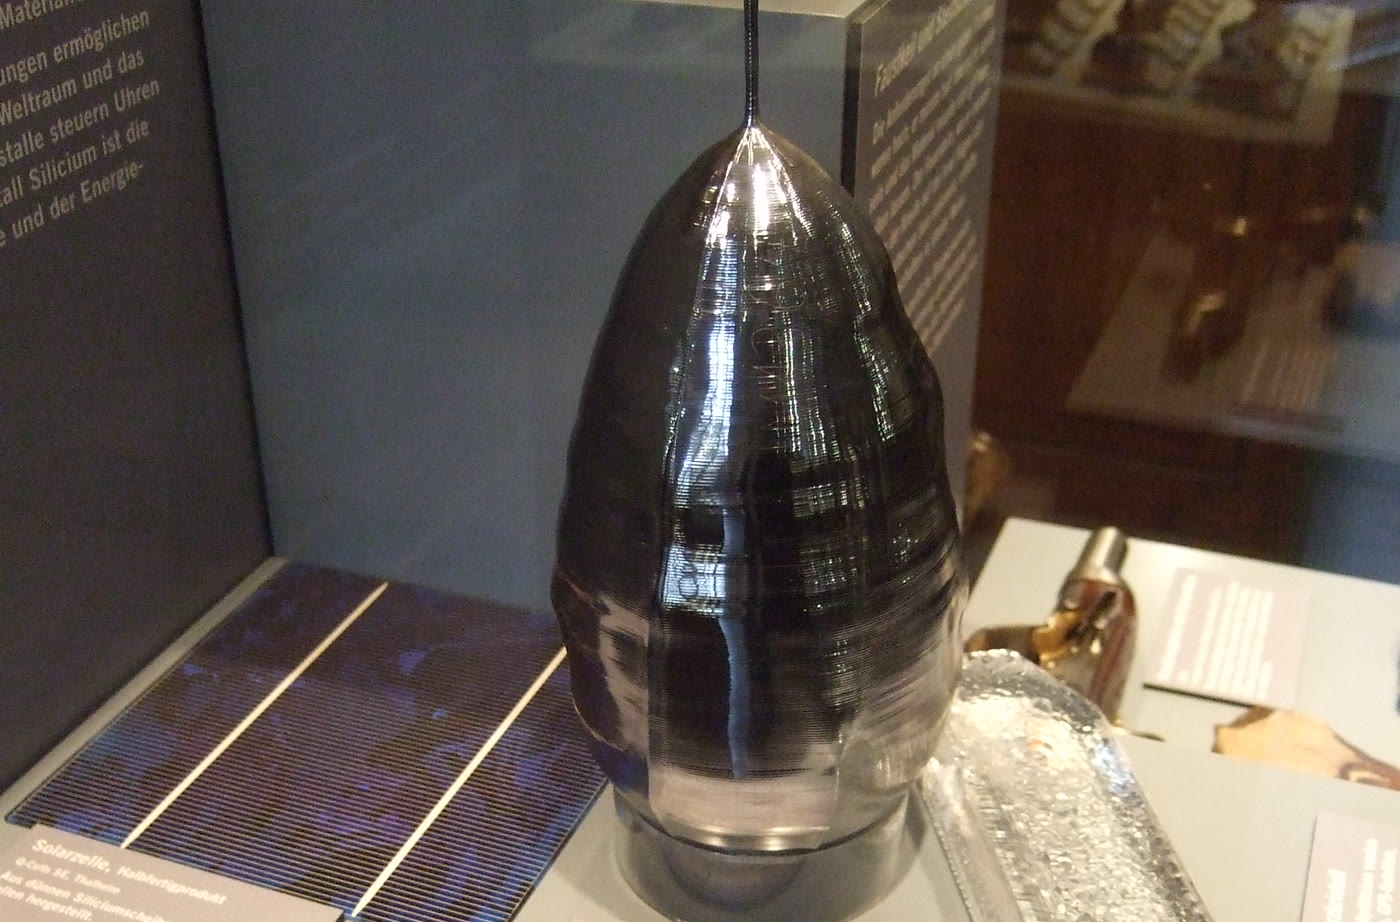
\includegraphics[width=0.5\linewidth]{images/book4/silicon-boule.jpg}

{\small Um monocristal de silício puxado do material fundido, mostrado ao lado de uma célula
solar feita de uma fatia de um cristal desse tipo. Fotografia: Sebastian Wallroth,
domínio público.}
\end{omfigure}

\begin{inthelab}[Crescer um cristal de silício]
No método de Czochralski, silício policristalino muito puro é fundido em um
cadinho de sílica sob argônio, um pouco acima de seu ponto de fusão, com o
\omterm{def:b3:solid-state:doping}{dopante} adicionado ao fundido. Um pequeno cristal-semente em uma haste giratória é mergulhado no
fundido e erguido lentamente: o silício se cristaliza sobre ele com a
orientação da semente, e a velocidade de puxamento e de rotação fixa o diâmetro. O lingote
é então serrado em lâminas (\textit{wafers}) com menos de um milímetro de espessura. O silano e os gases
\omterm{def:b3:solid-state:doping}{dopantes} fosfina e arsina usados nas etapas seguintes são pirofóricos ou muito tóxicos,
e são manipulados somente em sistemas industriais fechados.
\end{inthelab}

\section{Defeitos pontuais}

\begin{definition}[Defeitos pontuais]\label{def:b3:solid-state:defects}
Um \emph{defeito pontual}\index{defeito pontual} é um desvio em relação ao cristal
perfeito localizado em um sítio: uma lacuna, um átomo intersticial ou um átomo
estranho. Em um cristal iônico, um \emph{defeito de Schottky}\index{defeito de Schottky} é um
par de lacunas, uma de cátion e uma de ânion, cujos íons foram para a
superfície; um \emph{defeito de Frenkel}\index{defeito de Frenkel} é um par formado por uma
lacuna e o íon que a deixou, situado em um sítio intersticial.
\end{definition}

\begin{omfigure}
\begin{tikzpicture}[scale=0.62]
  \begin{scope}
  \foreach \i in {0,...,5} \foreach \j in {0,...,4} {
    \pgfmathtruncatemacro{\pty}{mod(\i+\j,2)}
    \ifnum\pty=0 \fill[omDef!70] (\i,\j) circle (0.2); \else \fill[omThm!25] (\i,\j) circle (0.38); \draw[omThm!60] (\i,\j) circle (0.38); \fi
  }
  \fill[white] (2,2) circle (0.45); \draw[dashed] (2,2) circle (0.3);
  \fill[white] (3,2) circle (0.45); \draw[dashed] (3,2) circle (0.38);
  \node[font=\small\bfseries] at (2.5,5.0) {Schottky (NaCl)};
  \end{scope}
  \begin{scope}[xshift=8cm]
  \foreach \i in {0,...,5} \foreach \j in {0,...,4} {
    \pgfmathtruncatemacro{\pty}{mod(\i+\j,2)}
    \ifnum\pty=0 \fill[black!45] (\i,\j) circle (0.2); \else \fill[omMeth!25] (\i,\j) circle (0.38); \draw[omMeth!60] (\i,\j) circle (0.38); \fi
  }
  \fill[white] (2,2) circle (0.3); \draw[dashed] (2,2) circle (0.22);
  \fill[black!45] (2.5,2.5) circle (0.2);
  \draw[->, thick] (2.1,2.1) -- (2.38,2.38);
  \node[font=\small\bfseries] at (2.5,5.0) {Frenkel (AgCl)};
  \end{scope}
\end{tikzpicture}

{\small \omterm{def:b3:solid-state:defects}{Defeitos pontuais} em uma camada de um cristal do tipo sal-gema (pontos pequenos: cátions;
círculos grandes: ânions; tracejado: lacunas). À esquerda: um par de Schottky, faltam um cátion
e um ânion. À direita: um par de Frenkel, um íon prata deslocado de seu sítio
para uma posição intersticial.}
\end{omfigure}

\begin{theorem}[Concentração de equilíbrio dos defeitos de Schottky]\label{thm:b3:solid-state:schottky}
Em um cristal MX de $N$ unidades de fórmula, o número $n$ de pares de Schottky no
equilíbrio, com entalpia de formação $\Delta H_S$ por par e $n \ll N$, é
\[
  \frac{n}{N} = \eu^{-\Delta H_S/2kT}.
\]
\end{theorem}

\begin{proof}
Criar $n$ pares custa $n\,\Delta H_S$ e dá uma entropia configuracional, a partir das
$\binom{N}{n}$ maneiras de escolher as lacunas de cátion e outras tantas para os ânions:
$S = 2k\ln\frac{N!}{n!(N - n)!}$. Com a fórmula de Stirling $\ln x! \approx x\ln x - x$,
\[
  G(n) = n\,\Delta H_S - 2kT\bigl[N\ln N - n\ln n - (N - n)\ln(N - n)\bigr].
\]
No equilíbrio, $\dd G/\dd n = 0$: $\Delta H_S - 2kT\ln\frac{N - n}{n} = 0$, logo $n/(N - n) = \eu^{-\Delta H_S/2kT}$, e $n/N$ para
$n \ll N$. A entropia vibracional dos defeitos, aqui desprezada, multiplica o
resultado por um fator constante.
\end{proof}

\begin{proposition}[Defeitos de Frenkel]\label{prop:b3:solid-state:frenkel}
Com $N$ íons da espécie móvel, $N_i$ sítios intersticiais disponíveis para eles e
$\Delta H_F$ a entalpia de formação de um par, o número de pares de Frenkel é $n =
\sqrt{NN_i}\,\eu^{-\Delta H_F/2kT}$ (para $n \ll N, N_i$).
\end{proposition}

\begin{proof}
A entropia passa a ser $S = k\ln\binom{N}{n} + k\ln\binom{N_i}{n}$, e a mesma minimização dá
\[
  \Delta H_F = kT\ln\frac{(N - n)(N_i - n)}{n^2} \approx kT\ln\frac{NN_i}{n^2},
\]
donde o resultado.
\end{proof}

A raiz quadrada mostra que os defeitos se formam em pares: como $n_i$ em um \omterm{def:b3:solid-state:classes}{semicondutor},
sua concentração tem metade da energia de formação no expoente. Os haletos
alcalinos formam sobretudo \omterm{def:b3:solid-state:defects}{defeitos de Schottky}; os haletos de prata, cujo
$\ce{Ag+}$, pequeno e polarizável, cabe entre os ânions, sobretudo \omterm{def:b3:solid-state:defects}{defeitos de Frenkel}.

\begin{definition}[Notação de Kröger--Vink]\label{def:b3:solid-state:kroger-vink}
A \emph{notação de Kröger--Vink}\index{notacao de Kroger--Vink@notação de Kröger--Vink} escreve um \omterm{def:b3:solid-state:defects}{defeito pontual}
como $\mathrm{A_S^c}$: A é a espécie no sítio (V para uma lacuna, $i$ como sítio
para um intersticial), S o sítio que ela ocupa no cristal perfeito, e c sua
carga em relação a esse sítio: $\bullet$ para cada unidade positiva, $'$ para cada unidade
negativa, $\times$ para nenhuma.
\end{definition}

Assim, $\mathrm{V_{Na}'}$ é uma lacuna de sódio (o $+1$ ausente deixa uma carga relativa $-1$),
$\mathrm{V_{Cl}^{\bullet}}$ uma lacuna de cloreto, $\mathrm{Ag_i^{\bullet}}$ um íon prata intersticial, $\mathrm{Ca_{Na}^{\bullet}}$ um íon cálcio em um
sítio de sódio, $\mathrm{O_O^{\times}}$ um íon óxido em seu lugar. O equilíbrio de Schottky do NaCl é
$\text{nada} \rightleftharpoons \mathrm{V_{Na}' + V_{Cl}^{\bullet}}$, o equilíbrio de Frenkel do AgCl,
$\mathrm{Ag_{Ag}^{\times}} \rightleftharpoons \mathrm{Ag_i^{\bullet} + V_{Ag}'}$.

\begin{method}[Escrever uma equação de defeitos]\label{met:b3:solid-state:kroger-vink}
\begin{enumerate}
  \item Escreva o que é adicionado à matriz e os defeitos que isso cria.
  \item Balanço de sítios: a razão entre sítios de cátion e de ânion da matriz se conserva
        (as lacunas contam como sítios).
  \item Balanço de massa: os mesmos átomos dos dois lados (as lacunas não têm massa;
        os elétrons $e'$ e os \omterm{def:b3:solid-state:carriers}{buracos} $h^\bullet$ também não).
  \item Balanço de carga: as somas das cargas efetivas são iguais.
\end{enumerate}
\end{method}

\begin{example}[Ítria na zircônia]
Dissolver $\ce{Y2O3}$ em $\ce{ZrO2}$ põe dois $\ce{Y^3+}$ em sítios de $\ce{Zr^4+}$, cada um de carga relativa $-1$, e
três íons óxido em sítios de oxigênio; a razão da matriz, de um cátion para dois sítios de
oxigênio, exige quatro sítios de oxigênio para os dois cátions, de modo que um fica vazio:
\[
  \ce{Y2O3} \xrightarrow{\ce{ZrO2}} \mathrm{2\,Y_{Zr}' + 3\,O_O^{\times} + V_O^{\bullet\bullet}}.
\]
Sítios: 2 de cátion, 4 de oxigênio; massa: 2 Y e 3 O; carga: $2(-1) + 2 = 0$. Uma lacuna de
óxido para cada dois íons ítrio: é isso que faz da zircônia estabilizada com ítria
um condutor de íons óxido.
\end{example}

\begin{definition}[Centro de cor]\label{def:b3:solid-state:colour-centre}
Um \emph{centro de cor}\index{centro de cor} é um \omterm{def:b3:solid-state:defects}{defeito pontual} que absorve
luz visível, como um elétron preso em uma lacuna aniônica de um haleto
alcalino (um centro F), que colore um cristal de outro modo transparente.
\end{definition}

Aquecer o cloreto de sódio em vapor de sódio ou irradiá-lo cria centros F: o
elétron preso se comporta como uma \omterm{def:b3:quantum-model-systems:box}{partícula na caixa}, sendo a caixa do tamanho da lacuna, e
absorve no visível, tornando o cristal marrom-amarelado.

\section{Não estequiometria}

\begin{definition}[Compostos não estequiométricos]\label{def:b3:solid-state:non-stoichiometric}
Um \emph{composto não estequiométrico}\index{composto nao estequiometrico@composto não estequiométrico} é um
sólido cuja composição varia em uma faixa em torno de uma razão simples entre números
inteiros, sendo a diferença acomodada por \omterm{def:b3:solid-state:defects}{defeitos pontuais}.
\end{definition}

O óxido de ferro(II) nunca é exatamente $\ce{FeO}$: ele sempre tem falta de ferro,
$\mathrm{Fe_{1-x}O}$, com $x$ fixado pela temperatura e pela pressão de oxigênio em que foi preparado. Cada $\ce{Fe^2+}$ ausente é compensado por dois
$\ce{Fe^3+}$, que, na linguagem dos defeitos, são \omterm{def:b3:solid-state:carriers}{buracos} em sítios de ferro.

\begin{proposition}[Condutividade e pressão de oxigênio]\label{prop:b3:solid-state:brouwer}
Para um óxido deficiente em metal $\mathrm{M_{1-x}O}$ cujos defeitos são lacunas metálicas duplamente carregadas
compensadas por \omterm{def:b3:solid-state:carriers}{buracos}, a concentração de \omterm{def:b3:solid-state:carriers}{buracos}, e a condutividade, variam como
$p(\ce{O2})^{1/6}$. Para um óxido deficiente em oxigênio compensado por elétrons, elas variam como
$p(\ce{O2})^{-1/6}$.
\end{proposition}

\begin{proof}
A incorporação de oxigênio cria lacunas metálicas:
\[
  \tfrac12\ce{O2} \rightleftharpoons \mathrm{O_O^{\times} + V_M'' + 2\,h^{\bullet}}, \qquad K = \frac{[\mathrm{V_M''}][\mathrm h^\bullet]^2}{p(\ce{O2})^{1/2}}
\]
(a atividade de $\mathrm{O_O^{\times}}$ é 1). O
balanço de carga é $[\mathrm h^\bullet] = 2[\mathrm{V_M''}]$, logo $[\mathrm h^\bullet]^3 = 2K\,p(\ce{O2})^{1/2}$ e $[\mathrm h^\bullet] \propto p(\ce{O2})^{1/6}$. Para o
caso deficiente em oxigênio, $\mathrm{O_O^{\times}} \rightleftharpoons \tfrac12\ce{O2} + \mathrm{V_O^{\bullet\bullet} + 2\,e'}$, $[\mathrm e'] = 2[\mathrm{V_O^{\bullet\bullet}}]$, e as mesmas etapas dão $[\mathrm e'] \propto p(\ce{O2})^{-1/6}$.
A condutividade é proporcional à concentração de portadores.
\end{proof}

Um gráfico de $\log\sigma$ em função de $\log p(\ce{O2})$ indica, assim, quais defeitos dominam: sua inclinação,
$\pm 1/4$ ou $\pm 1/6$, depende de suas cargas.

\section{Condutores iônicos}

\begin{definition}[Condutores iônicos]\label{def:b3:solid-state:ionic-conductor}
Um \emph{condutor iônico}\index{condutor ionico@condutor iônico} é um sólido no qual a corrente
é transportada por íons que se movem através da rede. Um \emph{eletrólito
sólido}\index{eletrolito solido@eletrólito sólido} é um condutor iônico cuja condutividade eletrônica
é desprezível, de modo que ele pode separar os dois eletrodos de uma
célula eletroquímica.
\end{definition}

\begin{proposition}[Lei de Arrhenius da condução iônica]\label{prop:b3:solid-state:ionic-arrhenius}
Para íons que se movem por saltos entre sítios vizinhos sobre uma barreira $E_a$,
$\sigma T = A\,\eu^{-E_a/kT}$.
\end{proposition}

\begin{proof}[Demonstração parcial]
Um íon tenta saltos com uma frequência $\nu_0$ e tem êxito com probabilidade $\eu^{-E_a/kT}$,
de modo que seu coeficiente de difusão é $D = \tfrac16\nu_0 z a^2\eu^{-E_a/kT}$ para $z$ sítios vizinhos à
distância $a$ (passeio aleatório). A relação de Nernst--Einstein $\sigma = nq^2D/kT$ (admitida), para $n$
íons móveis de carga $q$ por unidade de volume, dá $\sigma T = (nq^2\nu_0za^2/6k)\,\eu^{-E_a/kT}$. A
concentração $n$ é fixada pela dopagem em um condutor extrínseco; quando ela própria é
criada termicamente, $E_a$ contém também metade da entalpia de formação.
\end{proof}

% ledger: trans:AgI
Três \omterm{def:b3:solid-state:ionic-conductor}{eletrólitos sólidos} mostram a gama de comportamentos. Na zircônia estabilizada com ítria, as
lacunas de óxido criadas pelo \omterm{def:b3:solid-state:doping}{dopante} permitem que os íons $\ce{O^2-}$ saltem; ela só conduz de modo útil
quando quente, a várias centenas de graus Celsius. Na alumina $\beta$, os íons sódio se movem em
planos pouco compactos entre blocos de espinélio, a base das baterias de
sódio--enxofre. O iodeto de prata se torna um condutor superiônico acima de \qty{146}{\celsius},
quando seus íons prata se distribuem por muito mais sítios do que há íons,
quase como um líquido dentro de uma rede rígida de iodeto. Os condutores de íons lítio
(granadas de zirconato de lítio e lantânio, sulfetos) são os eletrólitos das
baterias totalmente sólidas hoje em desenvolvimento.

\begin{omfigure}
\begin{tikzpicture}[font=\small, >=Stealth]
  \fill[omProp!25] (0,0) rectangle (2.4,3.2);
  \node[font=\scriptsize, align=center] at (1.2,0.6) {$\ce{ZrO2}$--$\ce{Y2O3}$\\ eletrólito sólido};
  \draw[black!60, line width=2.5pt] (-0.07,0) -- (-0.07,3.2);
  \draw[black!60, line width=2.5pt] (2.47,0) -- (2.47,3.2);
  \node[font=\scriptsize, align=center] at (-2.0,1.4) {gás de escape\\ $p(\ce{O2})$ baixa};
  \node[font=\scriptsize, align=center] at (4.4,1.4) {ar de referência\\ $p(\ce{O2}) = \qty{0.21}{bar}$};
  \node[font=\scriptsize, anchor=north] at (-0.07,-0.05) {Pt};
  \node[font=\scriptsize, anchor=north] at (2.47,-0.05) {Pt};
  \draw[->, thick, omThm] (2.0,1.9) -- (0.4,1.9) node[midway, above, font=\scriptsize] {$\ce{O^2-}$};
  \node[font=\scriptsize, anchor=west] at (2.65,2.75) {$\ce{O2 + 4e- -> 2O^2-}$};
  \node[font=\scriptsize, anchor=east] at (-0.25,2.75) {$\ce{2O^2- -> O2 + 4e-}$};
  \draw (-0.07,3.2) -- (-0.07,4.0) -- (0.85,4.0);
  \draw (2.47,3.2) -- (2.47,4.0) -- (1.55,4.0);
  \draw (1.2,4.0) circle (0.35) node {V};
\end{tikzpicture}

{\small O sensor de oxigênio de zircônia em corte: eletrodos porosos de platina
nas duas faces do \omterm{def:b3:solid-state:ionic-conductor}{eletrólito sólido}, um no gás de escape e o outro no ar.
Os íons óxido transportam a corrente através do eletrólito; a tensão mede a
razão entre as duas pressões de oxigênio.}
\end{omfigure}

\begin{history}[O transistor e o cristal puxado]
Em 1947, John Bardeen e Walter Brattain, no grupo de William Shockley nos Bell
Laboratories, construíram o primeiro transistor a partir de um cristal de germânio; os três
dividiram o Prêmio Nobel de Física de 1956. Os cristais vinham de um método que Jan
Czochralski encontrara em 1916 ao medir a velocidade de cristalização dos metais,
puxando um fio de estanho do metal fundido: adaptado ao germânio e depois ao silício,
ele ainda produz as lâminas de quase todos os circuitos integrados.
\end{history}

\section{Exercícios}

\begin{exercise}[$\star$]\label{exo:b3:solid-state:1}
Dê os seis níveis de Hückel de uma cadeia de seis átomos em unidades de $|\beta|$, e a
largura do intervalo que eles ocupam.
\end{exercise}

\begin{exercise}[$\star$]\label{exo:b3:solid-state:2}
Quantos elétrons comporta uma banda construída a partir dos orbitais s de $N$ átomos? Por que
o sódio e o magnésio são ambos metais?
\end{exercise}

\begin{exercise}[$\star$]\label{exo:b3:solid-state:3}
Estime o comprimento de onda da luz emitida por diodos de fosfeto de gálio
(\qty{2.26}{eV}) e de nitreto de gálio (\qty{3.4}{eV}), usando $\lambda \approx hc/E_g$.
\end{exercise}

\begin{exercise}[$\star$]\label{exo:b3:solid-state:4}
Escreva as equações de Kröger--Vink da dissolução de $\ce{CaCl2}$ em $\ce{NaCl}$ e de $\ce{Y2O3}$ em $\ce{ZrO2}$, e
verifique cada balanço.
\end{exercise}

\begin{exercise}[$\star\star$]\label{exo:b3:solid-state:5}
Com $N_c = \num{6.2e15}\,T^{3/2}$, $N_v = \num{3.5e15}\,T^{3/2}$ (em $\unit{cm^{-3}}$) e $E_g = \qty{1.125}{eV}$ para o silício a \qty{300}{K},
e $N_c = \num{1.98e15}\,T^{3/2}$, $N_v = \num{9.6e14}\,T^{3/2}$, $E_g = \qty{0.661}{eV}$ para o germânio, calcule $n_i$ para cada um, e sua
razão.
\end{exercise}

\begin{exercise}[$\star\star$]\label{exo:b3:solid-state:6}
O silício é dopado com $\qty{1.0e16}{cm^{-3}}$ de fósforo. Com $n_i = \qty{1.0e10}{cm^{-3}}$ a \qty{300}{K}, dê as
concentrações de elétrons e de \omterm{def:b3:solid-state:carriers}{buracos}.
\end{exercise}

\begin{exercise}[$\star\star$]\label{exo:b3:solid-state:7}
Para o cristal do \cref{exo:b3:solid-state:6}, quão acima do nível intrínseco fica
o \omterm{def:b3:solid-state:fermi}{nível de Fermi}?
\end{exercise}

\begin{exercise}[$\star\star$]\label{exo:b3:solid-state:8}
A entalpia de formação de um par de Schottky no NaCl é de cerca de \qty{2.3}{eV} (dados do
exercício). Calcule a fração de sítios vagos a \qty{800}{K} e o número de
pares em um mol.
\end{exercise}

\begin{exercise}[$\star\star$]\label{exo:b3:solid-state:9}
Uma amostra de óxido de ferro(II) (estrutura do sal-gema, quatro sítios de oxigênio por cela) tem
$a = \qty{430.0}{pm}$ e densidade de \qty{5.70}{g.cm^{-3}} (dados do exercício). Supondo
os sítios de oxigênio cheios, encontre $x$ em $\mathrm{Fe_{1-x}O}$.
\end{exercise}

\begin{exercise}[$\star\star\star$]\label{exo:b3:solid-state:10}
Um condutor de íons lítio tem $\sigma = \qty{1.0e-4}{S.cm^{-1}}$ a \qty{300}{K}, $\qty{7.8e-4}{S.cm^{-1}}$ a \qty{350}{K} e
$\qty{3.6e-3}{S.cm^{-1}}$ a \qty{400}{K} (dados do exercício). Encontre sua energia de ativação.
\end{exercise}

\begin{exercise}[$\star\star\star$]\label{exo:b3:solid-state:11}
Mostre que, em um óxido cujos defeitos dominantes são lacunas metálicas monocarregadas
$\mathrm{V_M'}$ compensadas por \omterm{def:b3:solid-state:carriers}{buracos}, a condutividade varia como $p(\ce{O2})^{1/4}$.
\end{exercise}

\begin{exercise}[$\star\star\star$]\label{exo:b3:solid-state:12}
No AgCl, o par de Frenkel tem uma entalpia de formação de cerca de \qty{1.4}{eV}, e há
dois sítios intersticiais por íon prata (dados do exercício). Calcule a fração
de íons prata em sítios intersticiais a \qty{600}{K}.
\end{exercise}

\section{Problema: O sensor de oxigênio em um escapamento}

\begin{problem}[{Problema de fim de semana --- o sensor de oxigênio em um escapamento: os
defeitos da zircônia estabilizada com ítria, sua condutividade iônica e sua temperatura de
operação, a tensão de Nernst da célula e a comutação entre gás de escape pobre e
rico}]
\label{pb:b3:solid-state:1}
% ledger: const:R, const:F, const:kB, const:e, const:NA, air:O2
O eletrólito do sensor é zircônia com 8.0\,mol\,\% de $\ce{Y2O3}$, de estrutura fluorita,
com quatro sítios de cátion e oito de oxigênio por cela cúbica, $a = \qty{514}{pm}$; um disco
de \qty{1.0}{mm} de espessura e \qty{0.20}{cm^2} de área separa o gás de escape do ar. Sua
condutividade segue $\sigma T = A\eu^{-E_a/kT}$ com $E_a = \qty{1.0}{eV}$ e $\sigma = \qty{0.030}{S.cm^{-1}}$ a \qty{800}{\celsius}. O gás de escape
pobre tem $p(\ce{O2}) = \qty{0.010}{bar}$, o rico, $p(\ce{O2}) = \qty{1.0e-20}{bar}$ (todos dados do problema).

\medskip\noindent\textbf{Parte I --- O eletrólito.}
\begin{enumerate}
  \item Escreva a equação de Kröger--Vink da dissolução de $\ce{Y2O3}$ em $\ce{ZrO2}$.
  \item Verifique seus balanços de sítios, de massa e de carga.
  \item Quantas lacunas de óxido são criadas por íon ítrio?
  \item Escreva a composição como $\mathrm{Zr_{1-x}Y_xO_{2-x/2}}$ e calcule $x$.
  \item Calcule a fração de sítios de oxigênio vagos.
  \item Calcule o número de lacunas por cela.
  \item Calcule a concentração de lacunas em $\unit{cm^{-3}}$.
\end{enumerate}

\medskip\noindent\textbf{Parte II --- Condutividade e temperatura.}
\begin{enumerate}[resume]
  \item Por que a condutividade cresce fortemente com a temperatura?
  \item Calcule $A$.
  \item Calcule $\sigma$ a \qty{700}{\celsius}.
  \item Calcule $\sigma$ a \qty{300}{\celsius}.
  \item Calcule a resistência do disco a essas duas temperaturas.
  \item A eletrônica exige uma resistência inferior a \qty{1}{k\ohm}: encontre a menor
        temperatura de operação.
  \item Por que esses sensores são equipados com um aquecedor?
\end{enumerate}

\medskip\noindent\textbf{Parte III --- A tensão de Nernst.}
\begin{enumerate}[resume]
  \item Escreva a reação de eletrodo do lado do ar, em notação comum e em
        \omterm{def:b3:solid-state:kroger-vink}{notação de Kröger--Vink}.
  \item Mostre que a tensão da célula é $E = (RT/4F)\ln\bigl(p_{\mathrm{air}}/p_{\mathrm{exh}}\bigr)$.
  \item Calcule $RT/4F$ a \qty{700}{\celsius}.
  \item Qual seria a tensão se o gás de escape contivesse ar?
  \item Calcule a variação de tensão por fator de dez em $p(\ce{O2})$.
\end{enumerate}

\medskip\noindent\textbf{Parte IV --- Pobre, rico e a comutação.}
\begin{enumerate}[resume]
  \item Calcule a tensão em gás de escape pobre a \qty{700}{\celsius}.
  \item Calcule a tensão em gás de escape rico a \qty{700}{\celsius}.
  \item Por que $p(\ce{O2})$ é tão pequena no gás de escape rico?
  \item O controle do motor comuta em \qty{0.45}{V}: a que pressão de oxigênio isso
        corresponde?
  \item Por que a tensão salta na razão ar/combustível estequiométrica, e como
        o controle do motor a utiliza?
  \item Enuncie o resultado: a tensão do sensor em gás de escape rico a \qty{700}{\celsius}.
\end{enumerate}
\end{problem}
